\chapter{Open Source Anonymous Credentials Benchmark Library}\label{chap6}
Anonymous Credentials lack a standardized, practical evaluation tool which will hinder adoption progress. I introduce an open-source library in Rust that benchmarks state-of-the-art Attribute-Based Anonymous Credential (ABC) schemes under consistent conditions. The field suffers from inconsistent comparisons—varying languages (e.g., Python, C++, Rust) and libraries (e.g., Arkworks, Ethereum PyEcc)—making it hard to assess schemes like BBS+ and PS fairly. Our work bridges this gap, offering practitioners a tool to understand functional differences and performance trade-offs while revealing how cryptographic optimizations enhance efficiency beyond theoretical predictions.

\section{Core Contributions}
My primary contribution is an open-source Rust library that implements and benchmarks leading ABC schemes (e.g., BBS+, PS, and their variants), providing a standardized framework for fair comparisons. Unlike prior evaluations, which lack consistency, our library ensures identical conditions—same hardware, security parameters, and libraries—highlighting the most efficient scheme for the critical ``Show + Verify'' operation (e.g., PS-UTT22 at 5.38 ms for 30 attributes, a 6.09x speedup over PS16). This tool also serves as an educational resource, helping practitioners explore constructions and select schemes for use cases like decentralized identity or Sybil-resistant voting.

My second contribution demonstrates the gap between theoretical and practical cryptography through three optimizations:
\begin{enumerate}
    \item \textbf{Schnorr Proofs with Multi-Scalar Multiplication (MSM):} I show that Schnorr proofs, often criticized as linear in attribute size, scale sublinearly in practice using MSM, challenging theoretical assumptions and boosting efficiency in New Generation Anonymous Credential schemes using $\G_1$ Schnorr proofs.
    
    \item \textbf{Batch Verification:} This batching technique aggregates multiple Schnorr proofs, cutting verification time by 50\% (e.g., useful in threshold systems), via random linear combinations—a practical speedup for multi-credential scenarios.
    
    \item \textbf{Optimized Pairings:} By leveraging Miller-Loop optimizations, I show pairing computation cost can be reduced,  improving pairing-based credential performance.
\end{enumerate}

These findings, validated in our library, extend beyond ABCs, offering insights for broader cryptographic applications.


% Anonymous credential systems promise privacy-preserving identity solutions, yet practitioners often lack accessible tools to understand the practical differences between constructions like Schnorr-based proofs and pairing-based systems. Existing literature focuses heavily on theoretical complexity, leaving an educational gap in functional implementation details—such as what systems can or cannot do in real-world scenarios and how they perform under specific use cases. To address this, we developed an open-source library framework in Rust, implementing state-of-the-art (SOTA) anonymous credential constructions and benchmarking them against each other.

% This library serves as a standardized toolkit, enabling practitioners to explore how different systems handle use cases like decentralized identity or Sybil-resistant voting. By providing empirical performance data alongside functional insights, it clarifies trade-offs that theoretical analyses often overlook. For example, while academic papers may emphasize asymptotic complexity, our benchmarks reveal how optimizations shift these boundaries in practice, making the library a valuable educational and practical resource.

% Open-Source Benchmarking Framework

% We developed the first standardized open-source tooling for fair comparison of anonymous credential schemes, tackling inconsistencies in previous academic evaluations. This framework empowers researchers and industry practitioners to make informed implementation decisions using quantitative performance metrics, moving beyond unfair practical claims or purely theoretical analysis. By enabling reliable and consistent assessments, it accelerates both research advancements and practical adoption of privacy-preserving technologies.


\section{Standardized Anonymous Credential Benchmarking}



The Anonymous Credential field lacks standardized fair comparisons between the leading schemes (particularly BBS+ \cite{hutchison_constant-size_2006} and PS \cite{sako_short_2016}) and their newer variants \cite{camenisch_anonymous_2016}, \cite{tomescu_utt_2022}. Previous evaluations attempt to compare different schemes - although they might use consistent security parameters, variation in programming languages of the implementations (Python, C++, Rust), their underlying cryptography libraries (Arkworks, Ethereum PyEcc), and use of optimizations such as like Multi-Scalar Multiplication, Miller Loop Pairings, and Batch Techniques make fair comparison difficult to quantify. 


Anonymous Credentials serve as the backbone of privacy-preserving identity systems. 

Since their inception, Anonymous Credentials have primarily been academic works; however, with the increasing need for governments and organizations to migrate secure digital identity infrastructure, for example, in the US, 13 states have interoperable mobile digital driving licenses \cite{aamva_jurisdiction_nodate} with 30 more states in consideration, in addition to the EU's eIDAS framework requiring all member states to have such infrastructure by 2026 \cite{european_parliament_meps_2024}. In light of this, there are products from Microsoft \cite{microsoft_microsoft_2025}, AWS \cite{aws_verifiable_nodate}, and \cite{dock_labs_dock_nodate} enabling this technology in addition to standardisation efforts at W3C \cite{w3c_verifiable_2025, w3c_decentralized_2022}

Therefore, the urgent question is, what is this technology's privacy/security cost? There are constant trade-offs between privacy, security, functionality, and efficiency. Improving privacy and security comes at the expense of functionality and efficiency, and vice versa. To answer this, we have built an Open-Source Anonymous Credentials Benchmark Library and (thus far) built 6 different schemes with the goal of fair comparison. We show why previous benchmark analyses are not fair and furthermore we show our analysis of using efficient practical cryptography libraries.  

Previous deployments like IBM's Idemix \cite{camenisch_design_2002} and IRMA \cite{fischer-hubner_towards_2013} based on CL-Signatures \cite{camenisch_design_2002, cimato_signature_2003}, Hyperledger Fabric \cite{androulaki_hyperledger_2018} based on BBS+ \cite{hutchison_constant-size_2006}, Microsoft's U-Prove \cite{dunkelman_formal_2016} based on Brands' signatures \cite{brands_rethinking_2000}, were deployed in pilot programs \cite{dunkelman_formal_2016}, and proved that these systems were secure, private and feature-rich, but inefficient for widespread adoption. Their implementations were based on early constructions we label as "previous generation" and lacked efficient credential verification procedures required for the expected user experience needed for large-scale uptake, which we illustrate below.


\section{The Efficiency of New Generation Anonymous Credentials}
The performance comparison in Table \ref{tab:anon_creds_performance_old_gen_vs_new} demonstrates that newer anonymous credential schemes, such as BBS+2016 \cite{camenisch_anonymous_2016} and PS-UTT22 \cite{tomescu_utt_2022}, outperform older schemes like BBS+06 \cite{hutchison_constant-size_2006} and PS16 \cite{sako_short_2016} by shifting zero-knowledge proofs from the target group $(\mathbb{G}_T)$ to the source group ($\mathbb{G}_1)$\footnote{CL04 \cite{hutchison_signature_2004} is included in previous generation}. For 30 attributes, older schemes require computing over 3$\ell$, and 2$\ell$ $\G_T$ points respectively with Show and Verify times of 39.21 ms (BBS+06) and 32.78 ms (PS16). In comparison, newer schemes compute only in $\G_1$ and minimize pairings, achieving times of 5.72 ms and 5.38 ms—speedups of 6.85x and 6.09x, respectively. These improvements maintain full functionality, including selective disclosure and unlinkability, and rely on standard security assumptions, enhancing the practicality of anonymous credentials for digital identity systems.



\begin{table}[!ht]
\centering
\caption{Performance Comparison of Anonymous Credential Schemes for Show and Verify Algorithms ($\ell = 30$ Attributes)}
\label{tab:anon_creds_performance_old_gen_vs_new}
\begin{tabular}{|l|c|c|c|c|c|c|}
\hline
\textbf{Scheme} & \textbf{ZKPoK}  & \textbf{Show (ms)} & \textbf{Verify (ms)}  & \textbf{Show + Verify (ms)} & \textbf{Speedup} \\
\hline
BBS+06 & $\mathbb{G}_T$ & 12.91  & 26.30 & 39.21 & -- \\
\hline
BBS+2016 & $\mathbb{G}_1$ & 3.15  & 2.57 & 5.72 & 6.85x over BBS+ 06 \\
\hline
PS16 & $\mathbb{G}_T$ & 16.23  & 16.55 & 32.78 & -- \\
\hline
PS-UTT22 & $\mathbb{G}_1$ & 1.59  & 3.79 & 5.38 & 6.09x over PS16 \\
\hline
\end{tabular}
\end{table}




\begin{table}[htbp]\label{abc-performance-combined-table-chap6}
\centering
\caption{Performance of Anonymous Credential Operations (time in ms), $n$ is attribute count}
\begin{tabular}{@{}p{1.2cm}*{5}{>{\centering\arraybackslash}p{1.6cm}}@{}}
\toprule
$n$ & \cite{hutchison_constant-size_2006} & \cite{camenisch_anonymous_2016} & \cite{sako_short_2016} & \cite{tomescu_utt_2022} \ref{sec:formal_treatment_utt_rerand_sig} & Our Improved \ref{sec:formal_treatment_utt_rerand_sig} \\
\midrule
\multicolumn{6}{c}{\textbf{Obtain}}  \\
\midrule
\textbf{2} & 0.51 & 0.90 & 0.66 & 0.25 & \textbf{0.23} \\
\textbf{5} & 0.65 & 1.00 & 0.66 & 0.28 & \textbf{0.27} \\
\textbf{10} & 0.67 & 1.13 & 0.82 & 0.36 & \textbf{0.31} \\
\textbf{15} & 0.78 & 1.26 & 0.87 & 0.37 & \textbf{0.36} \\
\textbf{20} & 0.86 & 1.38 & 0.94 & \textbf{0.41} & \textbf{0.41} \\
\textbf{30} & 1.07 & 1.63 & 1.11 & 0.51 & \textbf{0.49} \\
\midrule
\multicolumn{6}{c}{\textbf{Issue}}  \\
\midrule
\textbf{2} & 1.25 & \textbf{0.72} & 1.48 & 1.27 & 2.99 \\
\textbf{5} & 1.66 & \textbf{0.75} & 1.79 & 1.66 & 3.31 \\
\textbf{10} & 2.33 & \textbf{0.83} & 2.54 & 2.35 & 4.00 \\
\textbf{15} & 2.98 & \textbf{0.84} & 3.23 & 3.03 & 4.64 \\
\textbf{20} & 3.96 & \textbf{0.90} & 3.79 & 3.66 & 5.88 \\
\textbf{30} & 4.97 & \textbf{0.94} & 5.16 & 5.10 & 6.86 \\
\midrule
\multicolumn{6}{c}{\textbf{Show}}  \\
\midrule
\textbf{2} & 5.39 & 2.31 & 3.20 & \textbf{1.14} & 1.29 \\
\textbf{5} & 6.05 & 2.42 & 3.15 & \textbf{1.16} & 1.29 \\
\textbf{10} & 7.44 & 1.71 & 4.53 & \textbf{1.22} & 1.33 \\
\textbf{15} & 8.86 & 2.71 & 6.14 & 1.40 & \textbf{1.37} \\
\textbf{20} & 11.88 & 1.88 & 7.66 & \textbf{1.41} & 1.51 \\
\textbf{30} & 12.91 & 3.15 & 16.23 & \textbf{1.37} & 1.59 \\
\midrule
\multicolumn{6}{c}{\textbf{Verify}}  \\
\midrule
\textbf{2} & 7.59 & 2.18 & 4.57 & 2.47 & \textbf{1.79} \\
\textbf{5} & 9.25 & 2.25 & 5.52 & 2.73 & \textbf{2.01} \\
\textbf{10} & 11.09 & \textbf{2.25} & 7.10 & 3.16 & 2.44 \\
\textbf{15} & 13.96 & \textbf{2.30} & 8.62 & 3.47 & 2.72 \\
\textbf{20} & 16.93 & \textbf{2.34} & 9.88 & 3.84 & 3.21 \\
\textbf{30} & 26.30 & \textbf{2.57} & 16.55 & 4.67 & 3.79 \\
\midrule
\multicolumn{6}{c}{\textbf{Issuing Phase Total (Obtain + Issue)}}  \\
\midrule
\textbf{2} & 1.76 & 1.62 & 2.14 & \textbf{1.53} & 3.22 \\
\textbf{5} & 2.31 & \textbf{1.76} & 2.45 & 1.95 & 3.57 \\
\textbf{10} & 3.00 & \textbf{1.96} & 3.37 & 2.71 & 4.31 \\
\textbf{15} & 3.75 & \textbf{2.10} & 4.10 & 3.40 & 5.00 \\
\textbf{20} & 4.82 & \textbf{2.29} & 4.74 & 4.06 & 6.28 \\
\textbf{30} & 6.04 & \textbf{2.57} & 6.27 & 5.60 & 7.35 \\
\midrule
\multicolumn{6}{c}{\textbf{Showing Phase Total (Show + Verify)}}  \\
\midrule
\textbf{2} & 12.98 & 4.48 & 7.77 & 3.61 & \textbf{3.08} \\
\textbf{5} & 15.30 & 4.67 & 8.68 & 3.90 & \textbf{3.30} \\
\textbf{10} & 18.53 & 3.96 & 11.62 & 4.38 & \textbf{3.77} \\
\textbf{15} & 22.82 & 4.22 & 14.76 & 4.87 & \textbf{4.09} \\
\textbf{20} & 28.81 & 5.01 & 17.53 & 5.25 & \textbf{4.72} \\
\textbf{30} & 39.21 & 5.72 & 32.77 & 6.04 & \textbf{5.37} \\
\bottomrule
\end{tabular}
\end{table}














\subsection{Schnorr Proofs with Multi-Scalar Multiplication (MSM) are Sublinear}\label{sigma-protocol-analysis}

$\Sigma$-protocols, such as Schnorr proofs, are often characterized as having linear complexity with respect to the number of attributes. However, by leveraging multi-scalar multiplication (MSM)—an optimized algorithm widely available in cryptographic libraries—we demonstrate that these proofs achieve sublinear scaling in practice. MSM efficiently computes sums of scalar multiplications in elliptic curve groups, reducing the computational cost of proof generation and verification compared to naive approaches. This positively impacts the performance of Anonymous Credential schemes that leverage $\Sigma$-protocols. Figure \ref{fig:schnorr-benchmarks} provides benchmark results, illustrating the sublinear scaling as the number of attributes increases.

\begin{figure}[!htb]
    \centering
    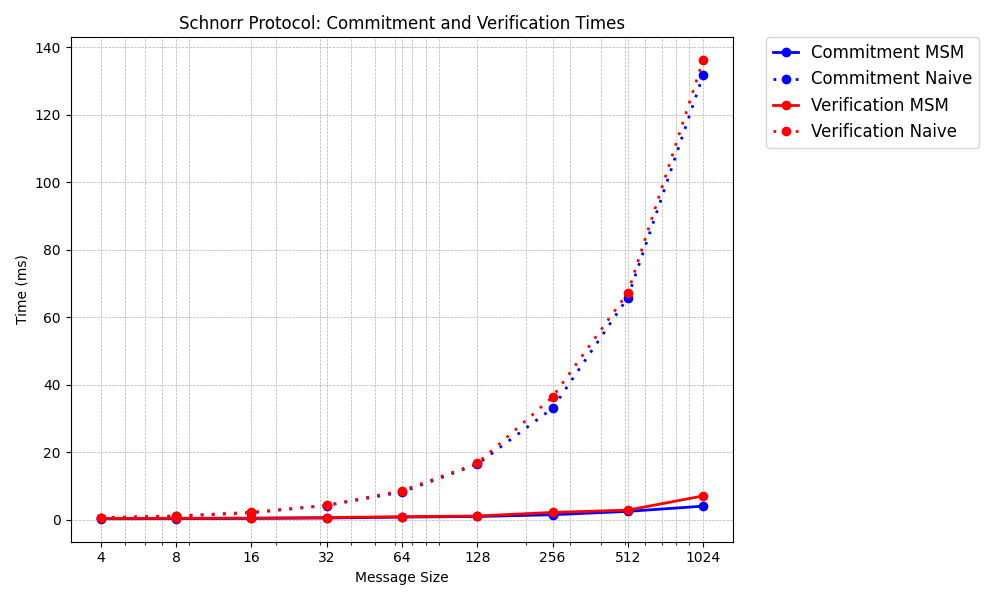
\includegraphics[width=0.75\linewidth]{schnorr_msm_no_msm.png}
    \caption{Schnorr Protocol - Practical Benchmarks with Multi-Scalar Multiplication}
    \label{fig:schnorr-benchmarks}
\end{figure}





\subsection{Pairing Protocols}

\begin{figure}
    \centering
    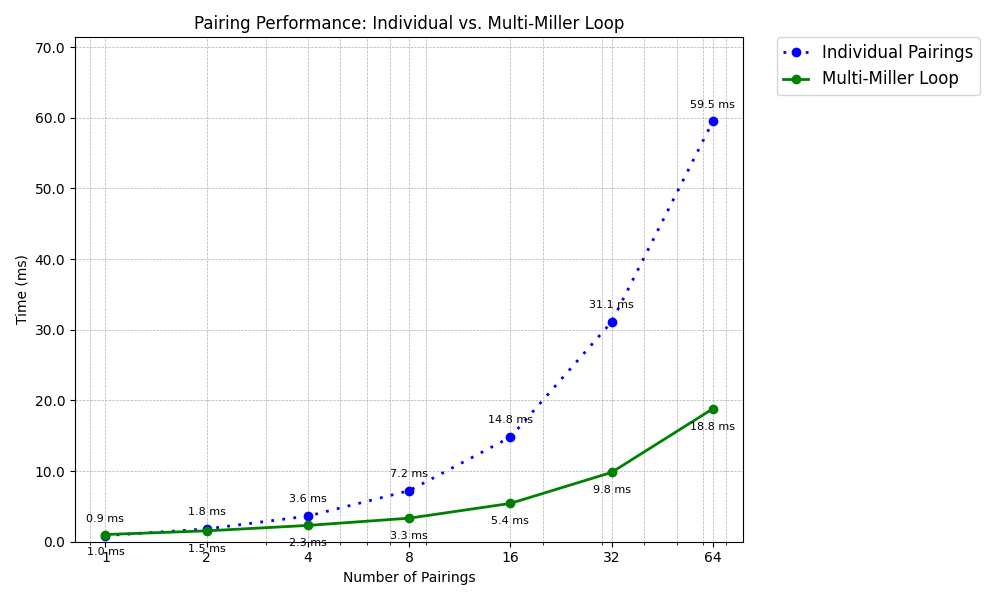
\includegraphics[width=0.75\linewidth]{pairing_comparison.png}
        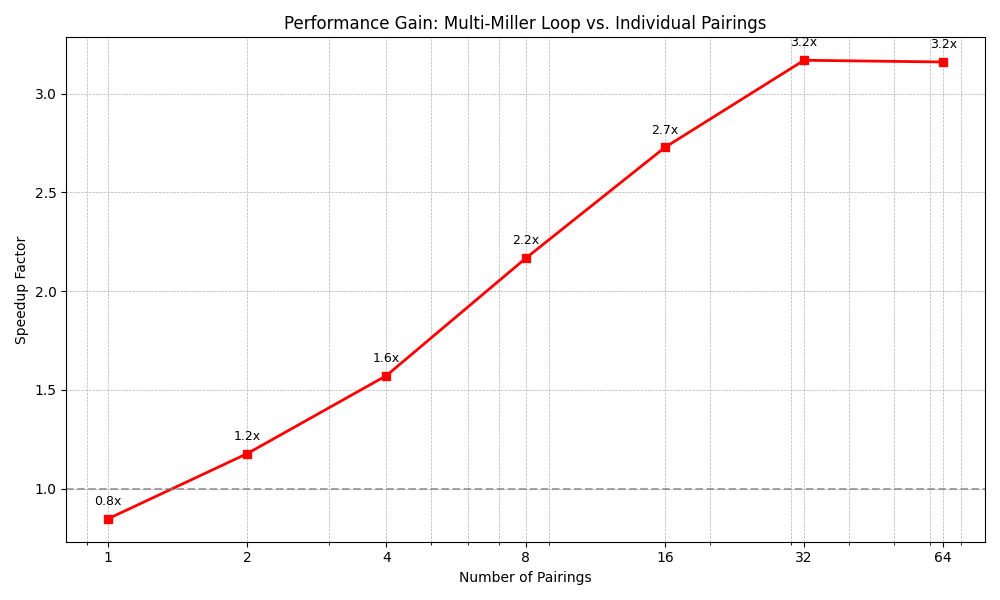
\includegraphics[width=0.75\linewidth]{pairing_comparison2.png}
    \caption{Elliptic Curve Pairings - Practical Benchmarks with Miller-Loop Intermediate Computation}
    \label{fig:elliptic_curve_pairings_speedup}
\end{figure}







\section{Impact and Conclusion}
This chapter delivers a standardized, accessible tool that empowers researchers and practitioners to evaluate ABC schemes empirically, accelerating their real-world adoption in digital identity systems (e.g., EU eIDAS, US mobile licenses). By debunking theoretical inefficiencies and showcasing practical gains—like sublinear Schnorr proofs and halved verification times—we provide a clearer picture of privacy/security costs. Future work could expand the library with more schemes and optimizations, enhancing its value. In summary, our contributions standardize comparisons, educate users, and optimize performance, paving the way for efficient, privacy-preserving identity solutions.




